% Chapter 'Evaluation'

\section{Project Methods}\footnote{This following part has, partially, been taken from our project, as we felt wasteful when practically rewriting information. We feel certain that the correct information can be conveyed in a responsible manner, given due self-acknowledgement.}
	\subsection{Hypothesis}
		To reiterate, our hypotheses were: \emph{$H_0:$ two knn-classifiers with a different k and otherwise identical, will not result in significantly different confusion tables} and \emph{$H_alt:$ two knn-classifiers with a different k and otherwise identical, will result in significantly different confusion tables.}
		
		In our project we tested several audio features and feature configurations.
		We tested window sizes of 20ms, 10ms, and 5ms; and window skips of 10ms, 5ms, 2ms respectively. This was the case for all features using windows: Mel Frequency Cepstral Coefficients (MFCC), Spectral Flux, Spectral Centroid, Spectral Skew, and Spectral Rolloff. Only the first 20 MFCC coefficients was used. The Root Mean Square (RMS) and Zero Crossing Rate (ZCR) was calculated over the entire sound.
		
		To determine if a difference in the independent variable $k$ had any significant effect on the resulting confusion tables (see Table \ref{table:eval:explanatory}), the chi squared test of association was used. We do have the independent variables 'feature' and 'feature configuration', although we know for a fact that they are used between-group, and that our groups (the sounds from the dataset) are exactly identical. That means that we can reliably say that we are manipulating only $k$, but just testing under different conditions unrelated to the classification method. Under each condition (each unique feature/configuration), the output confusion table from two knn-classifiers with only a different $k$, was compared. We compared all resulting unique pairs of tables using the chi squared test. Since we tested over 10 different $k$, but only on unique combinations of $K_1$ and $K_2$, the amount of tests done in total was $Tests = 10*9/2 = 45$. We have chosen that the null hypothesis can be disputed, if any calculated probability $p < \alpha$. Further, the Bonferroni correction\citep{bonferroni} was applied to $\alpha=0.05$, such that $\alpha=0.05/45 = 0.00\overline{1}$.
		
	\subsection{Measures}
		A confusion table was created for each test (each unique combination of variables). This was shown in percentages (or rather, on a scale from 0 and 1). Overall accuracy was calculated, along with precision, recall, and F-score for each sound class individually. For the sake of compactness, all the measures was included in an extended confusion table, as shown in the explanatory table \ref{table:eval:explanatory}. 
		The most important measure, for the sake of measuring our transcription system, would be the precision, that is, the amount of correctly transcribed sounds over the actual amount of that sound class.
		Recall should just be ignored, since we only test on the dataset, which means that we always test on all available samples of any given class, meaning that the observed amount would be the same as the total amount. This would be different, had the segmentation been part of the evaluation. When looking at results, we judged the performance primarily by accuracy and precision. Some of these measures could have been relevant to use for tests other than the chi squared, but that was not what we did at the time. We know that it is a valid and reliable measure, as we are only really looking for any difference, and as it is purely computational.

			\begin{table}
				\centering
				\begin{tabular}{|c | c | c | c | c |}
					\hline
				 & Real Class(1) & Real Class(2) & Real Class(3) & Precision\\ \hline
					Label(1)  & ... & ... & ... & ...\\ \hline
					Label(2)  & ... & ... & ... & ...\\ \hline
					Label(3) & ... & ... & ... & ...\\ \hline
					F-Score & ... & ... & ... & Accuracy \\ \cline{1-4}
				\end{tabular}
				\caption{$K=1$}
				\label{table:eval:explanatory}
			\end{table}
		
		
	\subsection{Data Collection}
	\label{sec:data-collecting}
	In order to build a system to transcribe beatboxing by amateurs, and in order to test the system, we had to create a dataset with many samples of beatboxing sounds. 
	Non-probability sampling was used to collect the data, in which 19 people participated, and it took place in the main building of Aalborg University Copenhagen. 
	
	The participants were placed in a chair surrounded by small partition walls (see cfigure \ref{data-collection-pic}) to limit noise from the surroundings. They were asked to produce 5-10 of each of the three types of sounds ('k', 's', 'hh'), and also to perform a self-improvised short mix of the sounds\footnote{This was done from a machine learning point-of-view, to better distinguish sounds with varying noise from other contemporary sounds.}
	
	To record the beatboxing sequences we used a e815-S dynamic cardioid microphone attached to an H4n portable recorder. The sampling rate was 96 kHz and 24 bit precision.
	
	The gathered data was collected on one track used as a database for our system. In order to utilize this database the sound file had to be manually annotated. This meant that for each sound its onset and duration was denoted and saved, and the type of sound labelled according to the three sound classes. This was done using Sonic Visualiser\footnote{\url{http://www.sonicvisualiser.org/}}, which generated a text file with the annotations.
	
	\begin{figure}[h]
		\begin{center}
			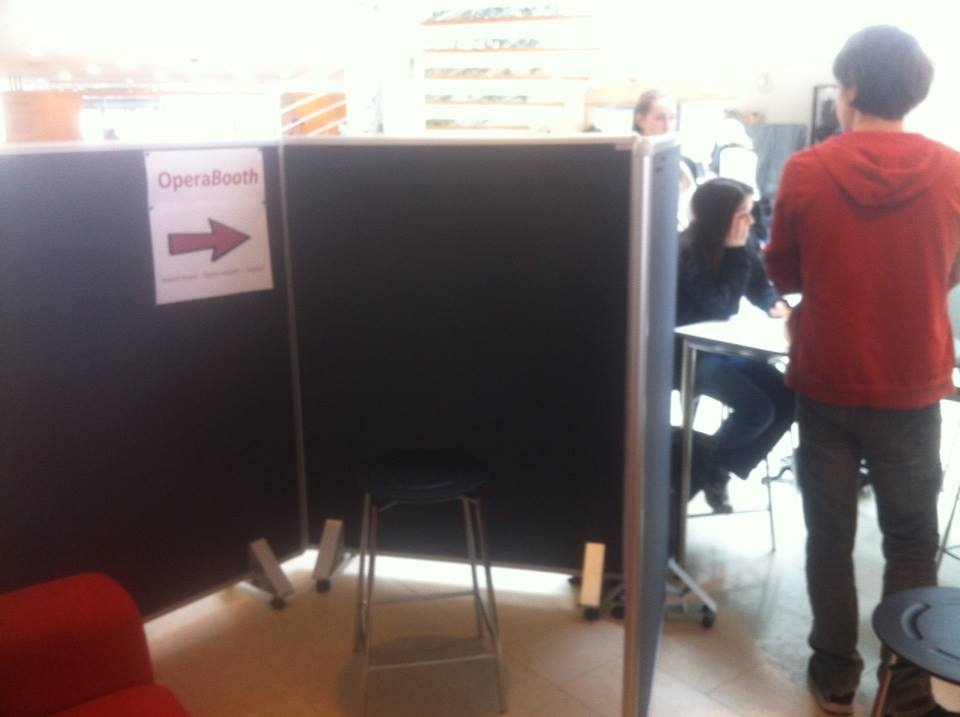
\includegraphics[height=5cm]{tex/dataset_collection.JPG}
			\caption{Data collection booth.}
			\label{data-collection-pic}
		\end{center}
	\end{figure}
	
	
	\subsection{Training and Test Sets}
		The annotated beatboxing sound dataset used, consists of sound segments, segmented based on the manual annotations. The training and test sets of sound samples for the KNN classifier were randomly chosen from the same population (the dataset). It was distributed between the training and test set in a 70\%/30\% ratio, accordingly, for each class. This means there will not be a fixed number of sounds for each class (neither total nor divided), but rather a fixed distribution between the number of training and test sounds for each class. We can do this instead of e.g. k-fold cross validation, due to scale of our collected dataset. The ratio was suggested by our supervisor\footnote{Bob L. Sturm} as a good balance for machine learning. The composition of the entire dataset has been summarized in table \ref{table:eval:datasetComposition}. 
		Furthermore, all sounds with a duration less than the windowsize used for feature calculation, were removed before testing, since calculation was impossible on such short sounds. This was done before splitting the dataset, such as to make sure we did not distort the 70/30 distribution.

		\begin{table}
			\centering
			\begin{tabular}{|l|r|r|}
					\hline
					Value  &  Count  & Percent \\ \hline
			      noise    &  150    & 10.19\% \\ \hline
			          k    &  466    & 31.66\% \\ \hline
			  undefined    &  130    &  8.83\% \\ \hline
			          s    &  331    & 22.49\% \\ \hline
			         hh    &  395    & 26.83\% \\ \hline
			      TOTAL    &  1472	 & 100.00\% \\ \hline

			\end{tabular}
			\caption{Dataset composition}
			\label{table:eval:datasetComposition}
		\end{table}	
			
 
\section{Project Results}
	
	For all results found, some interpretation of the data and statistics will be presented, although it will be kept short due to the breadth of configurations tested. Only the relevant results will be shown and discussed, based on the accuracy, however the other measures will be considered as well. Results of the $X^2$ tests will be summarized and explained. All data can be found in appendix \ref{app:res}. 

	%
	% RMS
	%
	
	\subsection{Root Mean Square}

	
		The best results using the RMS feature vector was observed using $K=9$ with accuracy 61.5\% (see appendix \ref{app:RMS:9}). Some configurations had slightly higher precision in classes 's' and 'hh', although this seems minimal (see e.g. appendix  \ref{app:rms:k6} and \ref{app:rms:k8}). The worst observed was using $K=1$, with accuracy 53.9\% see appendix \ref{app:RMS:1:worst}. All results from for the RMS feature can be found in appendix \ref{app:res:rms}. The $X^2$ test revealed no significant differences between any two $K$ (see all p in \ref{xlrms11}).

		
	%
	%	ZCR
	%
	
	\subsection{Zero Crossing Rate}
%		\begin{figure}
%			\centering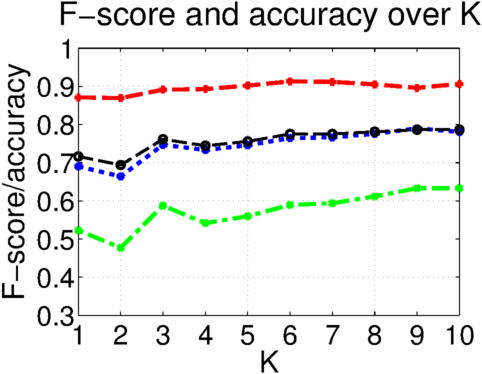
\includegraphics[width=0.3\textwidth]{tex/appendices/test/zcr11FP.png}
%			\centering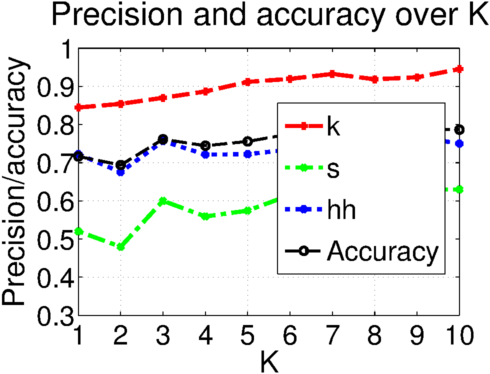
\includegraphics[width=0.3\textwidth]{tex/appendices/test/zcr11_P.png}
%			\centering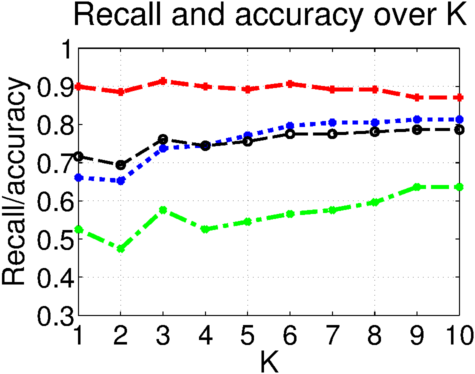
\includegraphics[width=0.3\textwidth]{tex/appendices/test/zcr11_R.png}
%			\label{fig:eval:zcr}
%			\caption{Plots over K for Zero Crossing Rate}
%		\end{figure}
%		
%		\begin{table}
%			\begin{subtable}[tbp]{0.45\textwidth}
%				\centering
%				\begin{tabular}{|c|c|c|c"c|}
%					\cline{2-5}
%					 \multicolumn{1}{c|}{} & \textbf{k}  & \textbf{s}  & \textbf{hh}  & Prec.\\ \hline
%					 \textbf{k} & \textcolor{red}{0.871} & 0.081 & 0.017 & 0.924\\ \hline
%					 \textbf{s} & 0.122 & \textcolor{red}{0.636} & 0.169 & 0.630\\ \hline
%					 \textbf{hh} & 0.122 & 0.283 & \textcolor{red}{0.814} & 0.768\\ \Xhline{2\arrayrulewidth}
%					 F & 0.896 & 0.633 & 0.790 & \textcolor{blue}{0.787}\\ \hline
%				\end{tabular}
%				\label{table:eval:zcrBest1}
%				\caption{$K=9$ (Best)}
%			\end{subtable}
%		
%			\begin{subtable}[tbp]{0.45\textwidth}
%				\centering
%				\begin{tabular}{|c|c|c|c"c|}
%					\cline{2-5}
%					 \multicolumn{1}{c|}{} & \textbf{k}  & \textbf{s}  & \textbf{hh}  & Prec.\\ \hline
%					 \textbf{k} & \textcolor{red}{0.871} & 0.051 & 0.017 & 0.945\\ \hline
%					 \textbf{s} & 0.122 & \textcolor{red}{0.636} & 0.169 & 0.630\\ \hline
%					 \textbf{hh} & 0.122 & 0.313 & \textcolor{red}{0.814} & 0.750\\ \Xhline{2\arrayrulewidth}
%					 F & 0.906 & 0.633 & 0.780 & \textcolor{blue}{0.787}\\ \hline
%				\end{tabular}
%				\label{table:eval:zcrBest2}
%				\caption{$K=10$ (Best)}
%			\end{subtable}
%			
%			\begin{subtable}[tbp]{0.45\textwidth}
%				\centering
%				\begin{tabular}{|c|c|c|c"c|}
%					\cline{2-5}
%					 \multicolumn{1}{c|}{} & \textbf{k}  & \textbf{s}  & \textbf{hh}  & Prec.\\ \hline
%					 \textbf{k} & \textcolor{red}{0.885} & 0.162 & 0.042 & 0.854\\ \hline
%					 \textbf{s} & 0.108 & \textcolor{red}{0.475} & 0.305 & 0.480\\ \hline
%					 \textbf{hh} & 0.108 & 0.364 & \textcolor{red}{0.653} & 0.675\\ \Xhline{2\arrayrulewidth}
%					 F & 0.869 & 0.477 & 0.664 & \textcolor{blue}{0.694}\\ \hline
%				\end{tabular}
%				\label{table:eval:zcrWorst}
%				\caption{$K=2$ (Worst)}
%			\end{subtable}
%			
%			\caption{Measures over K using ZCR}
%		\end{table}
		

		The best results using ZCR was a tie between $K=9$ (appendix \ref{app:zcr:best}) and $k=10$ (appendix \ref{app:zcr:best2}), both with accuracy 78.7\%. In the results from $K=9$, the precision of the hh is slightly better than in $K=10$ (75\% vs 67.5\%). In $K=10$, the precision of the kick is slightly better (94.6\% vs 92.4\%). The worst results was observed with $K=2$, having accuracy 69.4\%(appendix \ref{app-ZCR-Worst}). No tests were deemed significant by $X^2$ testing. See all $X^2$ results in appendix \ref{xlzcr11}.
		
	%	
	%	MFCC
	%	
		
	\subsection{Mel Frequency Cepstrum Coefficients}
%		\begin{figure}
%			\centering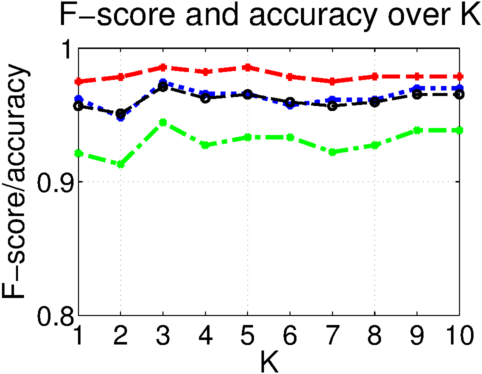
\includegraphics[width=0.3\textwidth]{tex/appendices/test/mfcc2010FP.png}
%			\centering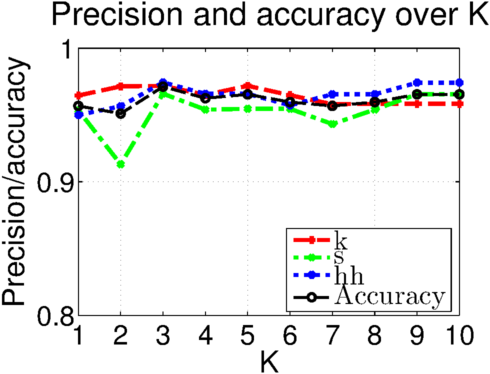
\includegraphics[width=0.3\textwidth]{tex/appendices/test/mfcc2010_P.png}
%			\centering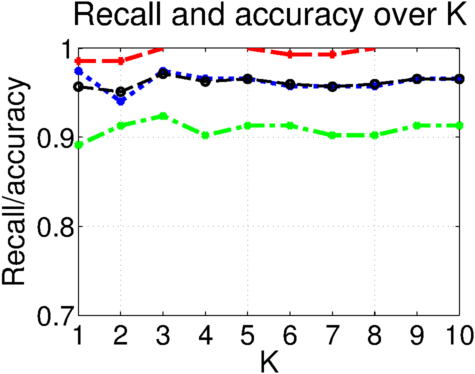
\includegraphics[width=0.3\textwidth]{tex/appendices/test/mfcc2010_R.png}
%			
%			\caption{Plots over K for MFCC with 20ms windows and 10ms window skips}
%		\end{figure}
%		\begin{figure}
%			\centering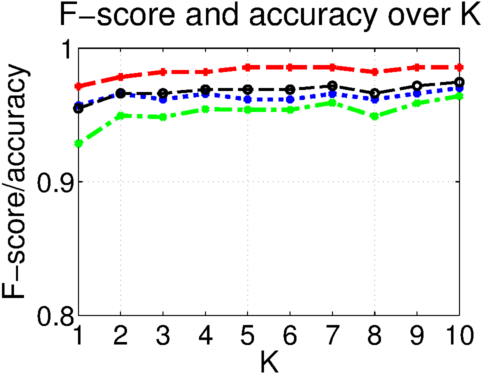
\includegraphics[width=0.3\textwidth]{tex/appendices/test/mfcc105FP.png}
%			\centering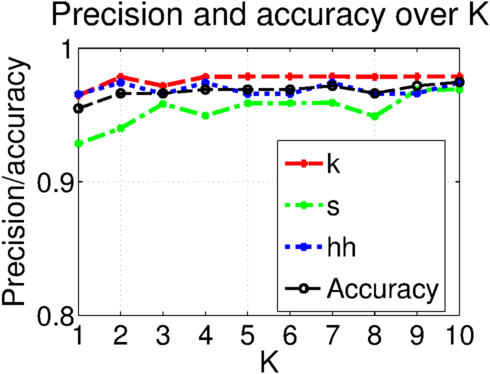
\includegraphics[width=0.3\textwidth]{tex/appendices/test/mfcc105_P.png}
%			\centering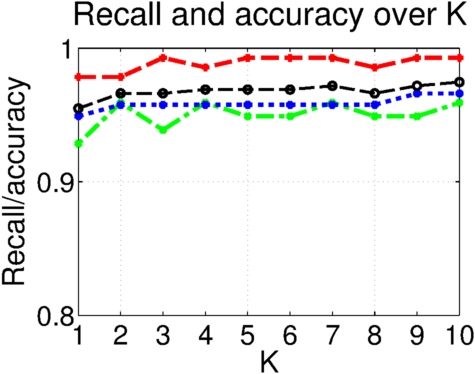
\includegraphics[width=0.3\textwidth]{tex/appendices/test/mfcc105_R.png}
%			
%			\caption{Plots over K for MFCC with 10ms windows and 5ms window skips}
%		\end{figure}
%		\begin{figure}
%			\centering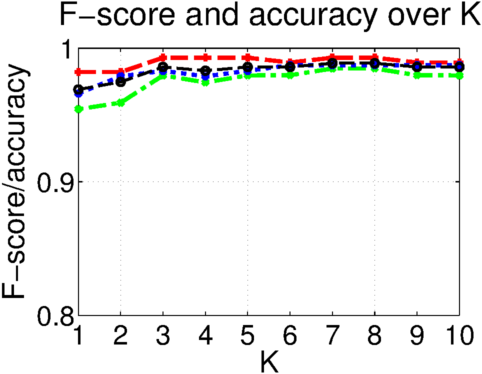
\includegraphics[width=0.3\textwidth]{tex/appendices/test/mfcc52FP.png}
%			\centering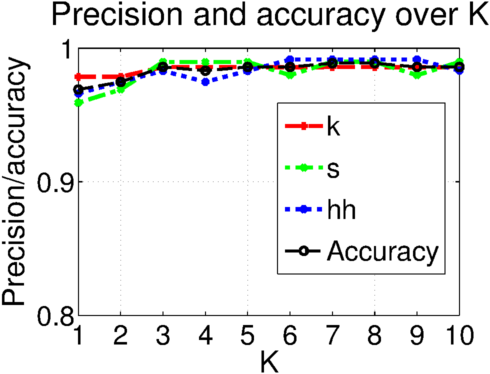
\includegraphics[width=0.3\textwidth]{tex/appendices/test/mfcc52_P.png}
%			\centering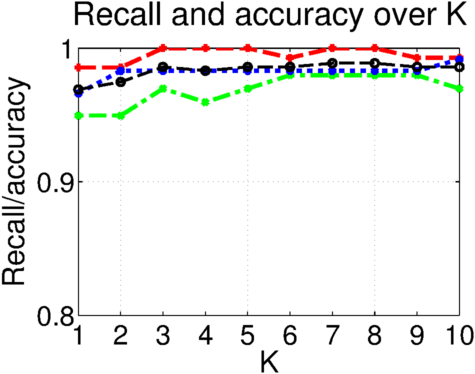
\includegraphics[width=0.3\textwidth]{tex/appendices/test/mfcc52_R.png}
%			
%			\caption{Plots over K for MFCC with 5ms windows and 2ms window skips}
%		\end{figure}\clearpage
%		
%		\begin{table}
%			\begin{subtable}[tbp]{0.45\textwidth}
%				\centering
%				\begin{tabular}{|c|c|c|c"c|}
%					\cline{2-5}
%					 \multicolumn{1}{c|}{} & \textbf{k}  & \textbf{s}  & \textbf{hh}  & Prec.\\ \hline
%					 \textbf{k} & \textcolor{red}{1.000} & 0.010 & 0.008 & 0.986\\ \hline
%					 \textbf{s} & 0.000 & \textcolor{red}{0.980} & 0.008 & 0.990\\ \hline
%					 \textbf{hh} & 0.000 & 0.010 & \textcolor{red}{0.983} & 0.991\\ \Xhline{2\arrayrulewidth}
%					 F & 0.993 & 0.985 & 0.987 & \textcolor{blue}{0.989}\\ \hline
%				\end{tabular}
%				\caption{$wSize=5ms, wSkip=2ms, K=7$}
%				\label{table:eval:mfccBest1}
%			\end{subtable}
%			\hfill
%			\begin{subtable}[tbp]{0.45\textwidth}
%				\centering
%				\begin{tabular}{|c|c|c|c"c|}
%					\cline{2-5}
%					 \multicolumn{1}{c|}{} & \textbf{k}  & \textbf{s}  & \textbf{hh}  & Prec.\\ \hline
%					 \textbf{k} & \textcolor{red}{1.000} & 0.010 & 0.008 & 0.986\\ \hline
%					 \textbf{s} & 0.000 & \textcolor{red}{0.980} & 0.008 & 0.990\\ \hline
%					 \textbf{hh} & 0.000 & 0.010 & \textcolor{red}{0.983} & 0.991\\ \Xhline{2\arrayrulewidth}
%					 F & 0.993 & 0.985 & 0.987 & \textcolor{blue}{0.989}\\ \hline
%				\end{tabular}
%				\caption{$wSize=5ms, wSkip=2ms, K=8$}
%				\label{table:eval:mfccBest2}
%			\end{subtable}
%			\hfill
%			\begin{subtable}[tbp]{0.45\textwidth}
%			\centering
%			\begin{tabular}{|c|c|c|c"c|}
%			\cline{2-5}
%			 \multicolumn{1}{c|}{} & \textbf{k}  & \textbf{s}  & \textbf{hh}  & Prec.\\ \hline
%			 \textbf{k} & \textcolor{red}{0.986} & 0.043 & 0.000 & 0.971\\ \hline
%			 \textbf{s} & 0.007 & \textcolor{red}{0.913} & 0.060 & 0.913\\ \hline
%			 \textbf{hh} & 0.007 & 0.043 & \textcolor{red}{0.940} & 0.957\\ \Xhline{2\arrayrulewidth}
%			 F & 0.978 & 0.913 & 0.948 & \textcolor{blue}{0.951}\\ \hline
%			\end{tabular}
%			\caption{$wSize=20ms, wSkip=10ms, K=2$}
%			\label{table:eval:mfccWorst}
%			\end{subtable}
%			
%			\caption{Measures over K using MFCC}
%		\end{table}
		

		Over all three configurations of the MFCC feature vector, the best performing were $K=7$ and $K=8$ with accuracies 98.9\%, when using a window size of 5ms and skip of 2ms (see appendix \ref{app:MFCC:7:best} and \ref{app:MFCC:8:best}). Some of the other results with the same parameters reach similar performance in regards to precision per class (see appendix \ref{tlmfcc52}). The worst performing, with 95.1\% accuracy, is using 20ms window size and 10ms skip with $K=2$ (see appendixs \ref{app:Mfcc:2:worst}). It still has better precision for kick than some others(e.g. $K=4$ or $K=6$), but some have similar hh precision (e.g. $K=1$ or $K=6$). No $X^2$ results were considered significant (although some came quite close; see appendix \ref{xlmfcc52}).
		
	%
	% SC
	%
	\subsection{Spectral Centroid}

		Using the Spectral Centroid feature, the best configuration found, with accuracy 82.8\% was 10ms windows and 5ms window skips, and $K=9$, as shown in appendix \ref{app:sc:9:best}. Some results show similar or better precision in some classes, e.g. $K=8$. The worst accuracy seen, was usisng 20ms window size, 10ms window skip, and $K=2$, with accuracy 73.8\%, as shown in table \ref{app:SC:2:worst}. $X^2$-test revealed no significant differences (see all in appendix \ref{app:res:sc}).
		
				
	% 
	% SS
	%
	\subsection{Spectral Skew}
			
%		\begin{figure}
%			\centering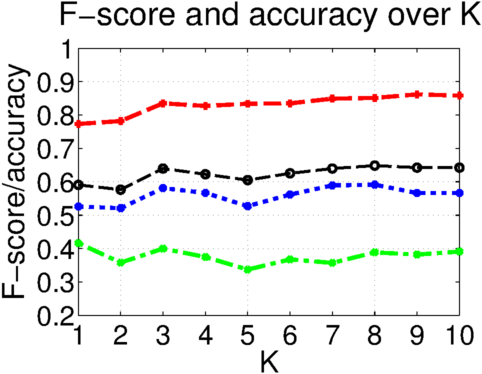
\includegraphics[width=0.3\textwidth]{tex/appendices/test/sskew2010FP.png}
%			\centering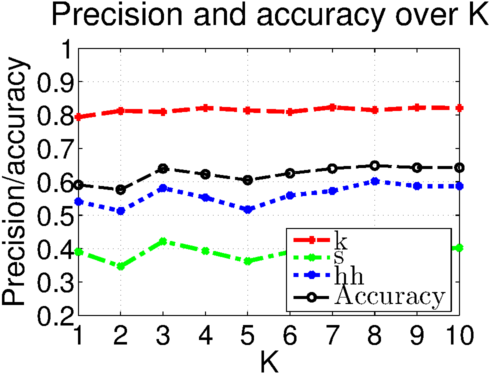
\includegraphics[width=0.3\textwidth]{tex/appendices/test/sskew2010_P.png}
%			\centering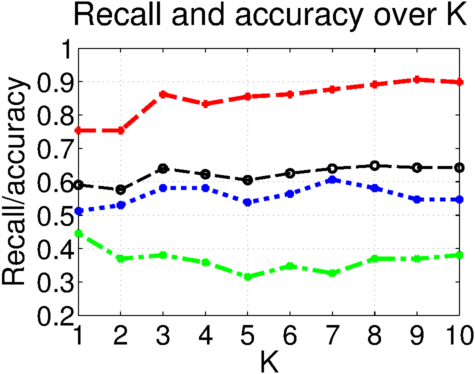
\includegraphics[width=0.3\textwidth]{tex/appendices/test/sskew2010_R.png}
%			
%			\caption{Plots over K for Spectral Skew with 20ms windows and 10ms window skips}
%		\end{figure}
%		
%		\begin{figure}
%			\centering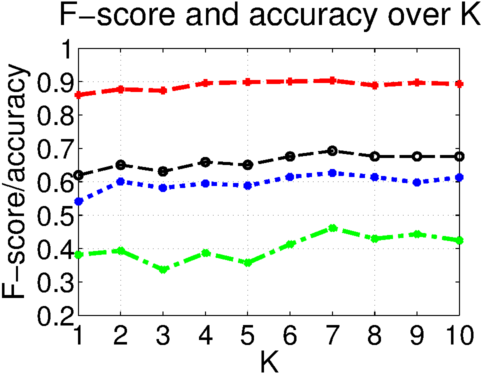
\includegraphics[width=0.3\textwidth]{tex/appendices/test/sskew105FP.png}
%			\centering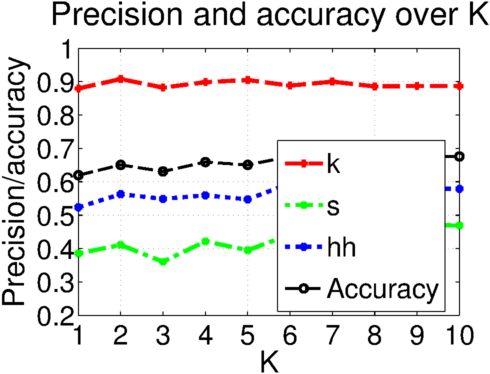
\includegraphics[width=0.3\textwidth]{tex/appendices/test/sskew105_P.png}
%			\centering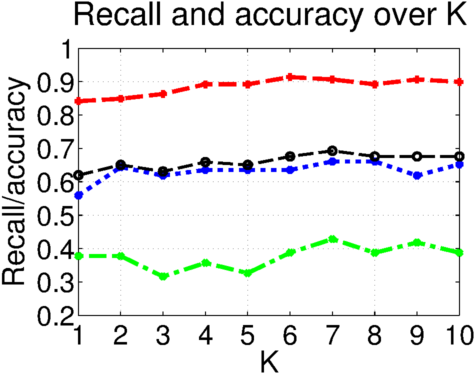
\includegraphics[width=0.3\textwidth]{tex/appendices/test/sskew105_R.png}
%				
%				\caption{Plots over K for Spectral Skew with 10ms windows and 5ms window skips}
%		\end{figure}
%		\begin{figure}
%			\centering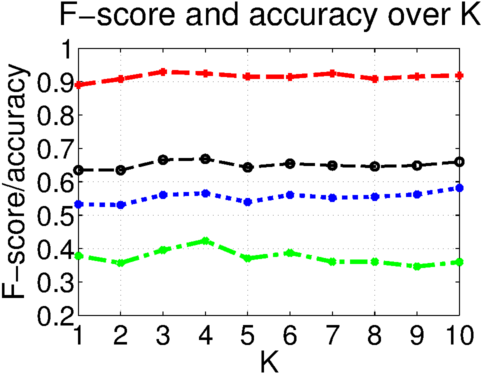
\includegraphics[width=0.3\textwidth]{tex/appendices/test/sskew52FP.png}
%			\centering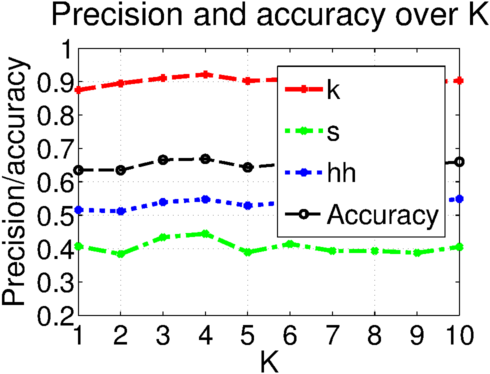
\includegraphics[width=0.3\textwidth]{tex/appendices/test/sskew52_P.png}
%			\centering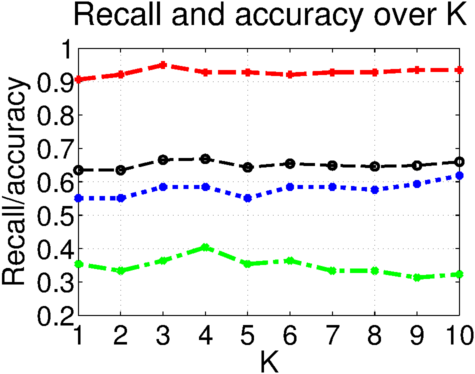
\includegraphics[width=0.3\textwidth]{tex/appendices/test/sskew52_R.png}
%				
%				\caption{Plots over K for Spectral Skew with 5ms windows and 2ms window skips}
%		\end{figure}\clearpage
%		
%		\begin{table}
%			\begin{subtable}[h]{0.45\textwidth}
%				\centering
%				\begin{tabular}{|c|c|c|c"c|}
%					 \cline{2-5}
%					 \multicolumn{1}{c|}{} & \textbf{k}  & \textbf{s}  & \textbf{hh}  & Prec.\\ \hline
%					 \textbf{k} & \textcolor{red}{0.942} & 0.031 & 0.008 & 0.970\\ \hline
%					 \textbf{s} & 0.058 & \textcolor{red}{0.786} & 0.288 & 0.647\\ \hline
%					 \textbf{hh} & 0.058 & 0.184 & \textcolor{red}{0.703} & 0.822\\ \Xhline{2\arrayrulewidth}
%					  F & 0.956 & 0.710 & 0.758 & \textcolor{blue}{0.820}\\ \hline
%				\end{tabular}
%				\caption{$wSize=10ms, wSkip=5ms, K=7$}
%				\label{table:eval:skewBest}
%			\end{subtable}
%			\hfill
%			\begin{subtable}[h]{0.45\textwidth}
%				\centering
%				\begin{tabular}{|c|c|c|c"c|}
%					\cline{2-5}
%					 \multicolumn{1}{c|}{} & \textbf{k}  & \textbf{s}  & \textbf{hh}  & Prec.\\ \hline
%					 \textbf{k} & \textcolor{red}{0.964} & 0.081 & 0.008 & 0.937\\ \hline
%					 \textbf{s} & 0.036 & \textcolor{red}{0.768} & 0.280 & 0.667\\ \hline
%					 \textbf{hh} & 0.036 & 0.152 & \textcolor{red}{0.712} & 0.848\\ \Xhline{2\arrayrulewidth}
%					 F & 0.950 & 0.714 & 0.774 & \textcolor{blue}{0.826}\\ \hline
%				\end{tabular}
%				\caption{$wSize=5ms, wSkip=2ms, K=7$}
%				\label{table:eval:skewKicker}
%			\end{subtable}
%			\hfill
%			\begin{subtable}[h]{0.45\textwidth}
%				\centering
%				\begin{tabular}{|c|c|c|c"c|}
%					\cline{2-5}
%					 \multicolumn{1}{c|}{} & \textbf{k}  & \textbf{s}  & \textbf{hh}  & Prec.\\ \hline
%					 \textbf{k} & \textcolor{red}{0.920} & 0.163 & 0.009 & 0.888\\ \hline
%					 \textbf{s} & 0.072 & \textcolor{red}{0.446} & 0.239 & 0.519\\ \hline
%					 \textbf{hh} & 0.072 & 0.391 & \textcolor{red}{0.752} & 0.704\\ \Xhline{2\arrayrulewidth}
%					 F & 0.904 & 0.480 & 0.727 & \textcolor{blue}{0.738}\\ \hline
%				\end{tabular}
%				\caption{$wSize=20ms, wSkip=10ms, K=2$}
%				\label{table:eval:skewWorst}
%			\end{subtable}
%			\caption{Measures over K using Spectral Skewness}
%		\end{table}
		

		The most accurate result using Spectral Skew was 82\%, was $K=7$ with 10ms window size and 5ms window skip, as shown in appendix \ref{app:SS:7:best}. Some other tests was more precise on kicks (e.g. Spectral Skew with 5ms window and 2ms window skip, with $K=7$, see \ref{app:SS:7:kickbest}). The least accurate result was $K=2$, using 20ms window size, 10ms window skip (see appendix \ref{app:SS:2:worst}). $X^2$-test did not show any significant results.
	
	%
	% SF
	%
	\subsection{Spectral Flux}
		
%		\begin{figure}
%		
%			\label{figJitter}
%			\centering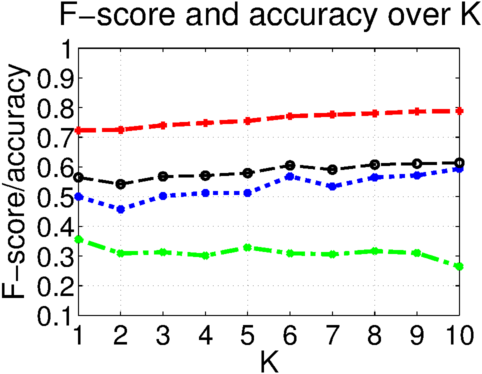
\includegraphics[width=0.3\textwidth]{tex/appendices/test/sflux2010FP.png}
%			\centering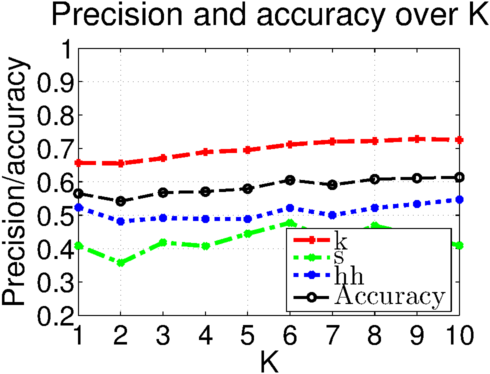
\includegraphics[width=0.3\textwidth]{tex/appendices/test/sflux2010_P.png}
%			\centering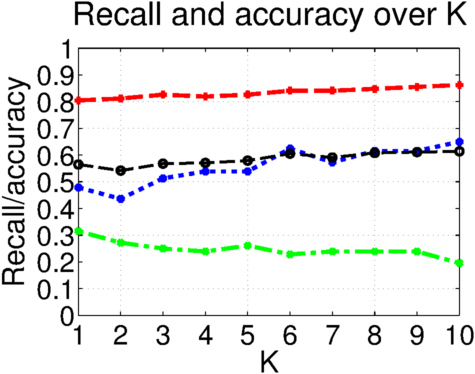
\includegraphics[width=0.3\textwidth]{tex/appendices/test/sflux2010_R.png}
%			
%			\caption{Plots over K for Spectral Flux with 20ms windows and 10ms window skips}
%		\end{figure}
%		\begin{figure}
%		
%		
%			\centering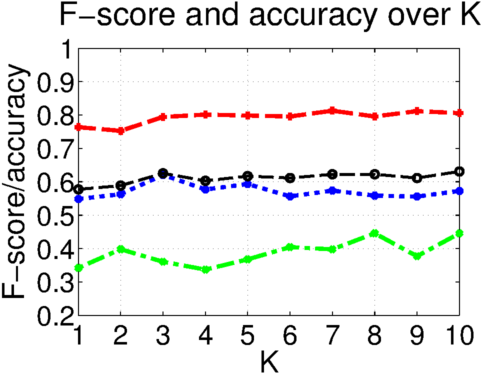
\includegraphics[width=0.3\textwidth]{tex/appendices/test/sflux105FP.png}
%			\centering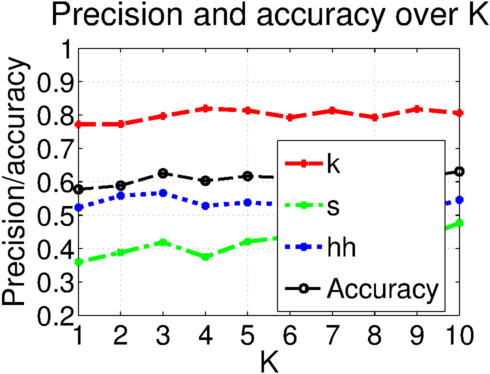
\includegraphics[width=0.3\textwidth]{tex/appendices/test/sflux105_P.png}
%			\centering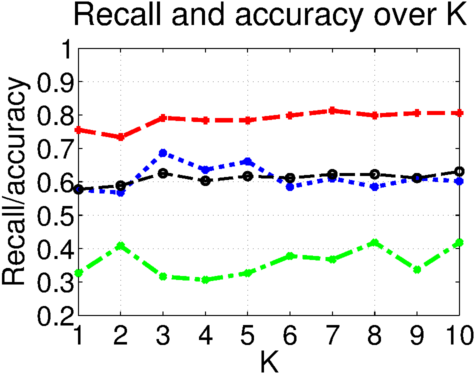
\includegraphics[width=0.3\textwidth]{tex/appendices/test/sflux105_R.png}
%				
%				\caption{Plots over K for Spectral Flux with 10ms windows and 5ms window skips}
%		\end{figure}
%		\begin{figure}
%		
%		
%			\centering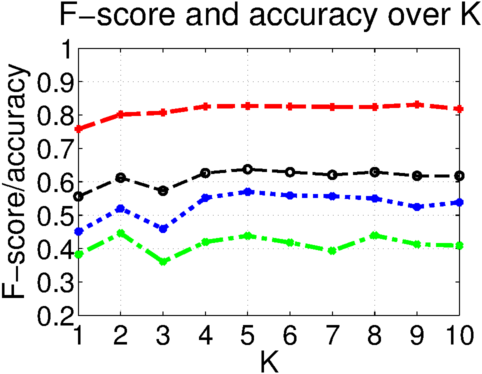
\includegraphics[width=0.3\textwidth]{tex/appendices/test/sflux52FP.png}
%			\centering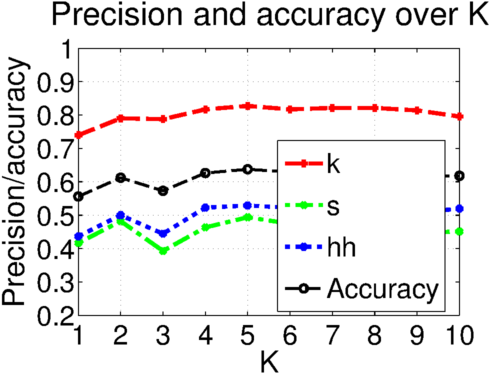
\includegraphics[width=0.3\textwidth]{tex/appendices/test/sflux52_P.png}
%			\centering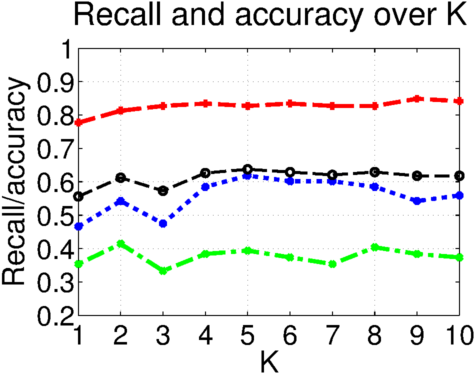
\includegraphics[width=0.3\textwidth]{tex/appendices/test/sflux52_R.png}
%				
%				\caption{Plots over K for Spectral Flux with 5ms windows and 2ms window skips}
%		\end{figure}
%		
%		\begin{table}
%			\begin{subtable}[h]{0.45\textwidth}
%				\centering
%				\begin{tabular}{|c|c|c|c"c|}
%					\cline{2-5}
%					 \multicolumn{1}{c|}{} & \textbf{k}  & \textbf{s}  & \textbf{hh}  & Prec.\\ \hline
%					 \textbf{k} & \textcolor{red}{0.827} & 0.121 & 0.102 & 0.827\\ \hline
%					 \textbf{s} & 0.050 & \textcolor{red}{0.394} & 0.280 & 0.494\\ \hline
%					 \textbf{hh} & 0.050 & 0.485 & \textcolor{red}{0.619} & 0.529\\ \Xhline{2\arrayrulewidth}
%					 F & 0.827 & 0.438 & 0.570 & \textcolor{blue}{0.638}\\ \hline
%				\end{tabular}
%				\caption{$wSize=5ms, wSkip=2ms, K=5$}
%				\label{table:eval:fluxBest}
%			\end{subtable}
%			\hfill
%			\begin{subtable}[h]{0.45\textwidth}
%				\centering
%				\begin{tabular}{|c|c|c|c"c|}
%					\cline{2-5}
%					 \multicolumn{1}{c|}{} & \textbf{k}  & \textbf{s}  & \textbf{hh}  & Prec.\\ \hline
%					 \textbf{k} & \textcolor{red}{0.812} & 0.293 & 0.274 & 0.655\\ \hline
%					 \textbf{s} & 0.080 & \textcolor{red}{0.272} & 0.291 & 0.357\\ \hline
%					 \textbf{hh} & 0.080 & 0.435 & \textcolor{red}{0.436} & 0.481\\ \Xhline{2\arrayrulewidth}
%					 F & 0.725 & 0.309 & 0.457 & \textcolor{blue}{0.542}\\ \hline
%				\end{tabular}
%				\caption{$wSize=20ms, wSkip=10ms, K=2$}
%				\label{table:eval:fluxWorst}
%			\end{subtable}
%			
%			\caption{Measures over K using Spectral Flux}
%		\end{table}
		
		The most accurate results with the Spectral Flux feature vector, was with 5ms window size, 2ms window skip, and $K=5$ (appendix \ref{app:SF:5:best}), however several test configurations using other feature parameters, show better precision for the highhat. The worst in terms of accuracy is the Spectral Flux using 20ms windows and 10ms window skips, with $K=2$, see appendix \ref{app:SF:2:worst}.	$X^2$ showed no significant results.
